\part{运动产生}
\markboth{运动产生}{运动产生}

\chapter{肌肉生物学和力量}\label{chap:chap4}


孤身一人,我们能做的太少。
团结起来,我们能做的却很多。
\begin{flushright}
	————海伦$\cdot$凯勒
\end{flushright}


\begin{figure}[!htb]
	\centering
	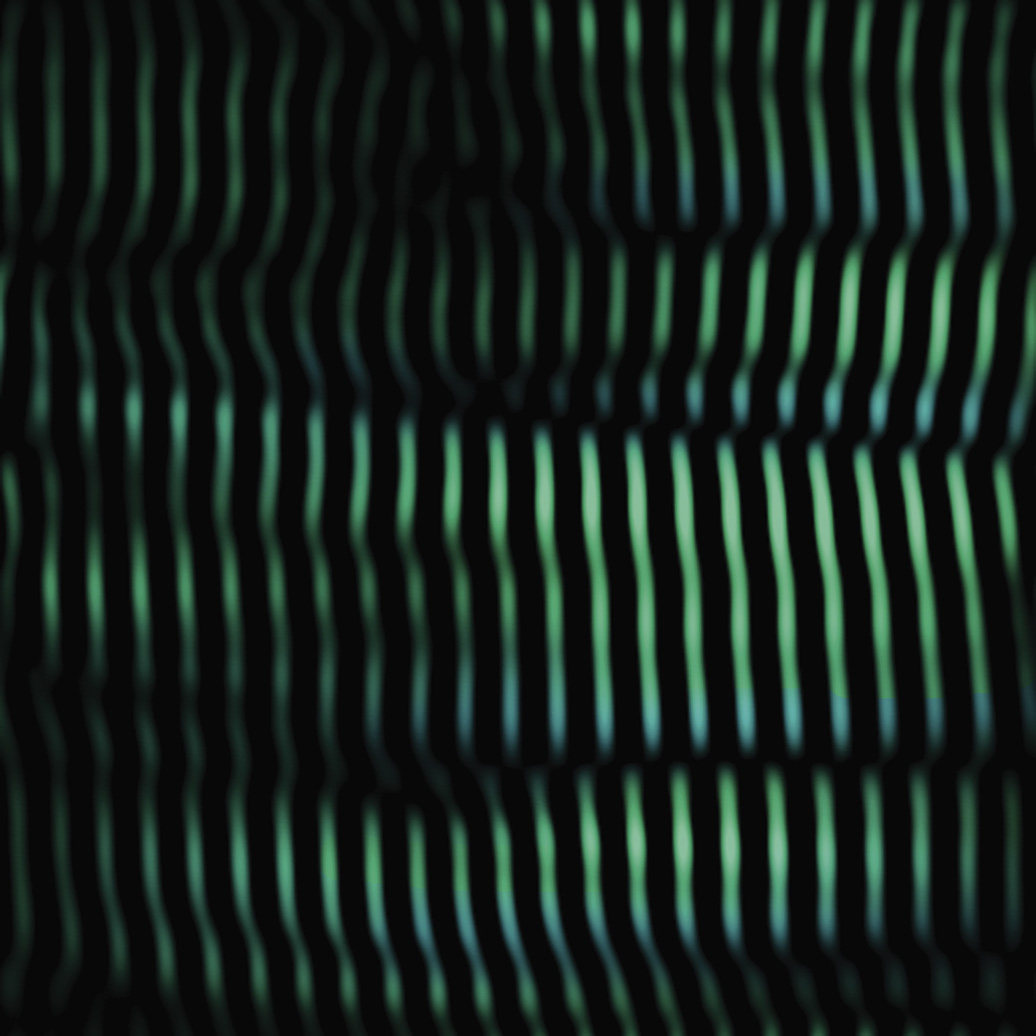
\includegraphics[width=1.0\linewidth]{chap4/4_0}
	% 加星号(*)表示不加编号
	\caption*{ \label{fig:4_0}}
\end{figure}


伦敦皇家学会拥有350年的历史,拥有近200年的传统,每年都会邀请科学家进行公开演讲,并经常进行一些简单的实验。
1952年,其中一项实验成为了热议话题。


两辆固定自行车朝向相反,并通过一条链条连接在一起,当一辆自行车向前踩踏板时,另一辆自行车的踏板就会向后移动(图~\ref{fig:4_1})。


\begin{figure}[!htb]
	\centering
	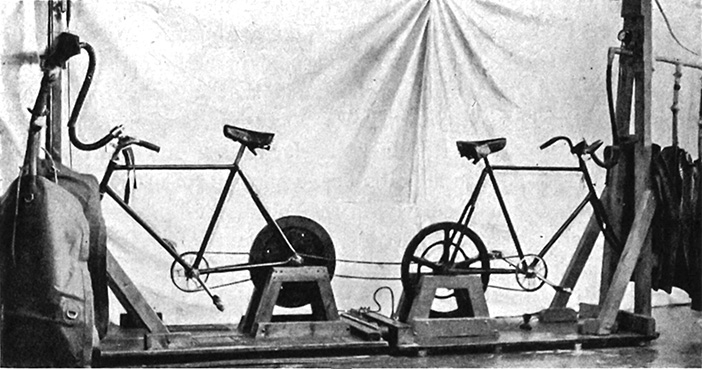
\includegraphics[width=1.0\linewidth]{chap4/4_1}
	\caption{Abbott 等人 (1952) 描述的推拉装置。 \label{fig:4_1}}
\end{figure}


一辆自行车上坐着一位娇小的女子,名叫布伦达$\cdot$比格兰,是肌肉疲劳研究领域的权威专家。
另一辆自行车上坐着一位魁梧的年轻人,名叫默多克$\cdot$里奇,他嫁给了他的自行车“对手”。
演讲者是A$\cdot$V$\cdot$希尔,他因在肌肉产热方面的研究而获得了诺贝尔奖。


里奇听从指令,用尽全力向前蹬,而比格兰则用力蹬着脚蹬,阻止他继续蹬。
想象一下,当观众看到这位娇小的女子轻而易举地阻止了这位身材高大的男人蹬得更快时,他们会有多么惊讶。
很快,他便大汗淋漓,气喘吁吁,而比格兰却几乎毫不费力。
甚至连伦敦市长后来也过来试驾。
“这套设备后来被命名为‘推拉你’,以纪念杜立特医生那只永远不知道自己要往哪个方向跑的双头怪兽,”布伦达$\cdot$比格兰-里奇后来写道。


魔术?小把戏?
并非如此,但它确实表明,肌肉消耗能量和产生力量的方式并非显而易见。
肌肉做正功(例如,在向前蹬踏时充当“马达”)时,它们消耗的能量和产生的热量,比做负功(例如,在向前蹬踏时充当“刹车”)时要多。
一般来说,肌肉产生的力量和消耗的能量,很大程度上取决于它是缩短还是伸长。
希尔实验的经验教训至今仍在日常康复和阻力训练中得到应用。
正如我们将看到的,奇迹发生在分子层面。


本章和下一章将深入探究肌肉内部,探索其结构与功能之间的关系。
肌肉是神奇的生物马达,能够在瞬间悄无声息地产生数千牛顿的力量。
这些力量如此巨大,以至于你小腿的肌肉就能举起一辆小型汽车的尾部。
这些巨大的力量是由数万亿个纳米级分子马达共同作用产生的,这些马达将我们摄入食物中的化学能转化为机械能,使我们能够活动。
这一非凡的功能源于骨骼肌特化的细胞机制和高度组织化的层级结构(图~\ref{fig:4_2})。


\begin{figure}[!htb]
	\centering
	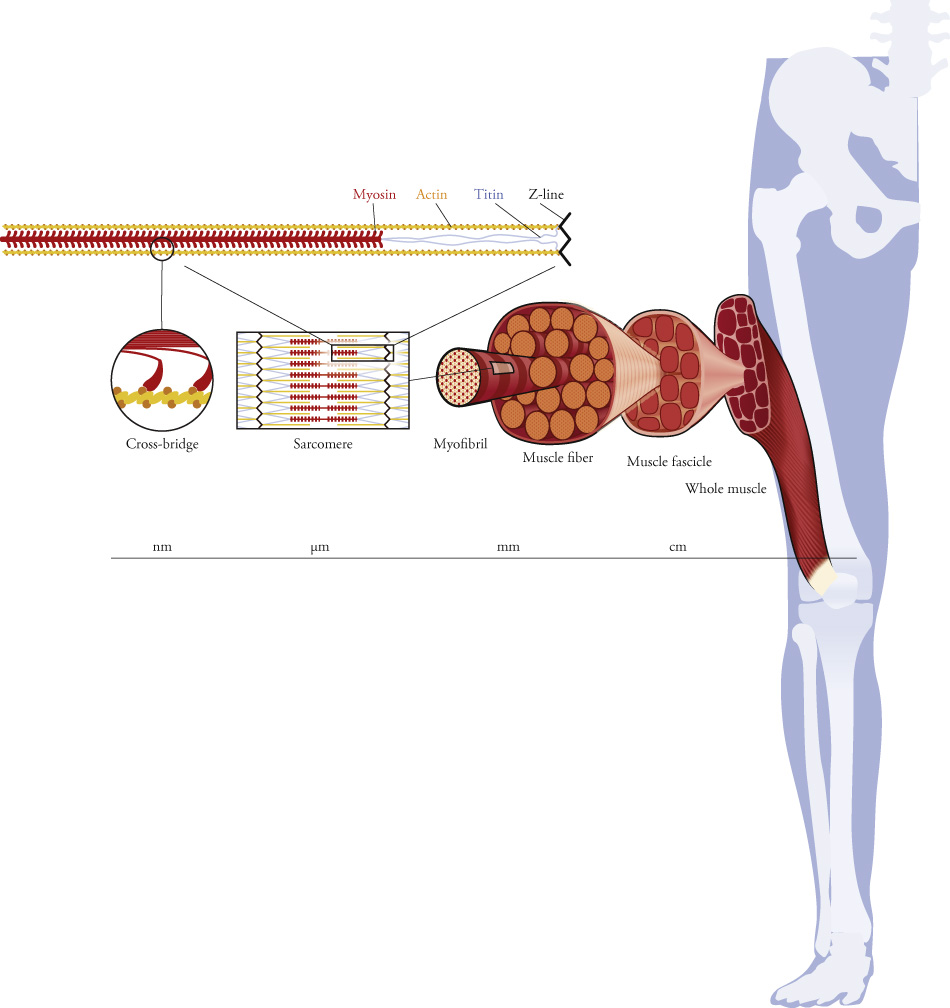
\includegraphics[width=1.0\linewidth]{chap4/4_2}
	\caption{肌肉的多尺度结构。
		骨骼肌具有层次结构,其中有被称为肌球蛋白的纳米级分子马达,每个肌球蛋白仅产生几皮牛顿的力,排列成肌节、肌原纤维、纤维、肌束和整个肌肉,在强力肌肉收缩期间可产生数千牛顿的力。 \label{fig:4_2}}
\end{figure}


接下来两章的组织将大致遵循肌肉的层级结构。
我们将首先在分子层面研究力量的产生过程。
接下来,我们将了解分子马达是如何被包裹在被称为肌节的亚细胞结构中的(活体人体肌节的第一张图像就是在我的手臂上拍摄的,并在本章的开篇图中展示)。
进一步深入,我们将了解单个肌肉细胞是如何被神经系统激活的,并了解“快肌纤维”和“慢肌纤维”之间的区别。
在第~\ref{chap:chap5}~章中,我们将从宏观层面研究肌肉在体内的排列方式,以及它们如何与肌腱(将肌肉力量传递到骨骼的结构)相互作用。


\section{肌肉结构}

从最基本的层面来说,肌肉通过两种细长蛋白质——肌动蛋白和肌球蛋白——的相互作用产生力量。
20世纪50年代初,休$\cdot$赫胥黎通过X射线显微镜发现,这些蛋白质平行排列,纤维交织,它们之间的连接被他称为“横桥”。
安德鲁$\cdot$赫胥黎(与休无亲属)同时用不同的方法发现了横桥。
赫胥黎和赫胥黎都怀疑横桥是产生力量的机制,并于1954年提出了一个关于这些分子马达如何工作的模型,我们将在下文中解释。
他们的模型一直是解释力量产生的基本范式,尽管随着更多实验数据的收集,该模型变得更加详细。


从尺寸上看,肌纤维排列成束,称为肌束,它们与肌肉纤维一样,长度可达数十厘米。
肌束的横截面积约为1毫米。
除了肌纤维外,肌束还包含称为细胞外基质的结缔组织,其中包括胶原蛋白、神经纤维和血管。
在健康的肌肉中,肌纤维紧密排列;
然而,在患病的肌肉中,肌纤维的横截面积可能较小,并被更多的细胞外基质和脂肪隔开。


肌束被更多结缔组织包围,并聚集在一起形成肌肉。
另一层结缔组织鞘被称为筋膜,包裹着肌肉并将其与其他肌肉隔开。
终止于每个肌束末端的肌纤维可以直接附着在骨骼上,但通常它们会连接到肌腱,肌腱随后附着在骨骼上。
肌腱插入肌肉的部分称为腱膜;肌腱在肌肉外部的部分通常称为游离肌腱。正如我们将在第五章中看到的,肌腱不仅通过向骨骼传递肌肉力量发挥着重要作用,还在伸展和回缩时储存和释放能量。




